%----------------------------------------------------------------------------
\chapter{Beszélőfelismerő modellek}
%----------------------------------------------------------------------------

\section{Voicemap}

A \emph{voicemap} egy nyílt forráskódú deep learning projekt beszélőfelismerő modellek létrehozására. A GitHub repository tartalmazza a modell kódját, a tanítást, különböző kísérleteket és egy optimalizált előre tanított modellt. Az implementációhoz \emph{Kerast} illetve újabb verziókban \emph{Pytorchot} használ.
\newline
\newline
A projekt célja, hogy későbbiekben egy olyan általános, pip által telepíthető csomag legyen, ami könnyen felhasználható beszélőfelismeréssel kapcsolatos feladatok elvégzésére.

\subsection{A projekt általános felépítése}

Mivel a saját alkalmazásomban felhasználtam és átalakítottam a projekt egyes részeit,
röviden bemutatom a felépítését.

\begin{itemize}
	\item \emph{models.py}: A konvolúciós enkóder létrehozása és a sziámi hálózat építését végzi el.
	\item \emph{librispeech.py}: Keras szekvencia osztály a librispeechből képzett tanítóadatok kezelésére. Fő paraméterei a következők:
	\begin{itemize}
		\item \emph{subsets}: Mely LibriSpeech adathalmazokat tartalmazza.
		\item \emph{seconds}: Az ennél rövidebb időtartamú hangmintákat figyelmen kívül hagyja.
		\item \emph{stochastic}: Sztochasztikus módban a mintákból véletlenszerűen vágjuk ki a \emph{seconds} hosszúságú darabot.
		\item \emph{pad}: Padding esetén a rövidebb hangmintákat nullával feltöltve a megadott méretre alakíthatjuk. Sztochasztikus mód esetén véletlenszerűen oszlik el a hangminta előtti és utáni nullák száma.
	\end{itemize}

	A két legfontosabb függvénye:
	
	\begin{itemize}
		\item \emph{build\_verification\_batch}: A sziámi hálózat teszteléséhez generál olyan batchet, amelyben az ugyanattól és az eltérő beszélőktől származó hangmintapárok száma azonos (50\%-50\%). A batch egy eleme két hangmintából és egy címkéből áll, ami jelzi, hogy egyazon vagy más-más beszélőktől származnak.
		\item \emph{build\_n\_shot\_task(k, n)}: Visszaad egy segédhalmazt $n$ mintával minden egyes $k$ beszélőtől és visszaad egy mintát, amiről a modellnek el kell döntenie, hogy melyik beszélőhöz tartozik.
	\end{itemize}
	\item \emph{utils.py}: Fő feladata az adatok preprocesszálása és a \emph{n\_shot\_task\_evaluation} függvény által az \emph{n-shot k-way} feladat kiértékelése. A few-shot kiértékeléshez alábbi argumentumokat adhatjuk meg:
	
	\begin{itemize}
		\item  \emph{model}: A tesztelendő modell.
		\item  \emph{dataset}: A tesztmintákat tartalmazó adathalmaz objektum.
		\item  \emph{preprocessor}: Előfeldolgozó függvény a minták csökkentett mintavételezésére és standardizálására.
		\item  \emph{num\_task}: A feladatok száma.
		\item  \emph{n}: Hány hangminta tartozik egy beszélőhöz a segédhalmazban.
		\item  \emph{k}: Ennyi beszélő, azaz osztály van a segédhalmazban.
		\item  \emph{network\_type}: Sziámi vagy klasszifikációs.
		\item  \emph{distance\_metric}: Sziámi hálózat esetén a hangvektorok közötti távolságmetrika.
	\end{itemize}
\end{itemize}

\subsection{Az implementált modellek}

A projekt két modellt vizsgál; egy sziámi neurális hálózatot és egy sima konvolúciósat klasszifikációval. Mindkét hálózat alapja alapja egy konvolúciós enkóder, amely a nyers hangmintákból kinyeri a jellemzőket és hangvektorokat állít elő belőlük. Az enkóder hálózat a több egymást követő konvolúciós blokk áll. Egy konvolúciós blokk felépítése a \ref{fig:conv_encoder_block} ábrán látható. Ezek egy konvolúciós rétegből és regularizációs
rétegekből tevődnek össze.

\begin{figure}[!ht]
	\centering
	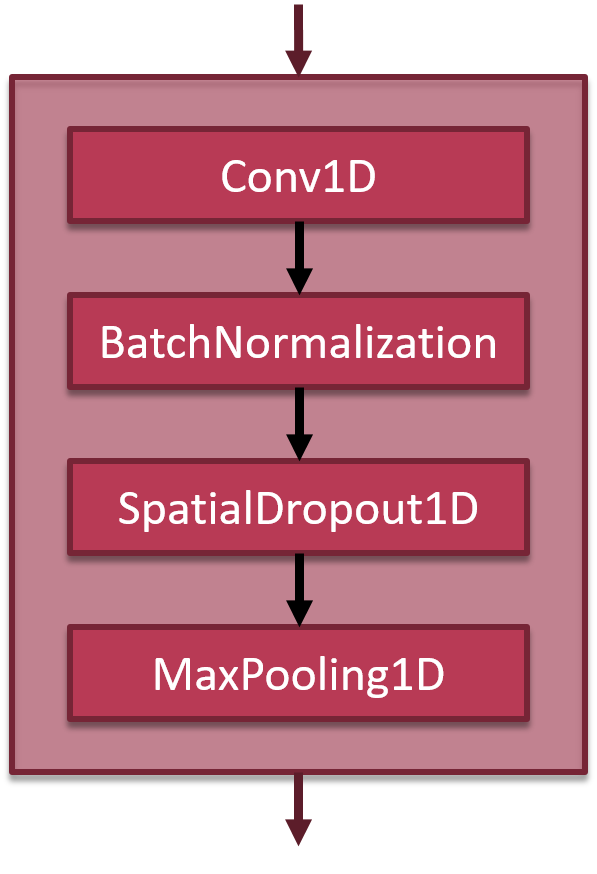
\includegraphics[width=80mm, keepaspectratio]{figures/conv_encoder_block.png}
	\caption{Egy konvolúciós enkóder blokk felépítése.}
	\label{fig:conv_encoder_block}
\end{figure}

\begin{itemize}
	\item Conv1D: 32-es méretű filterekkel, ahol a filterek száma arányosan nő azzal, hogy a blokk hányadik a sorban. Az aktivációs függvény \emph{ReLu}.
	\item BatchNormalization: Batchenként normalizálja az előző réteg kimeneteit úgy, hogy az átlag 0-hoz, a szórás 1-hez közelítsen. Regularizációra használják.
	\item SpatialDropout1D: Sima dropout réteg esetén az egyes neuronokat valamekkora valószínűséggel figyelmen kívül hagyjuk. Például egy [[1, 2, 3], [2, 3, 1]] tömbnek a kimenete sima dropout esetén lehet [[1, 0, 3], [0, 3, 1]], itt teljesen függetlenek egymástól a kinullázások. Spatial dropout esetén az adott dimenzió mentén mindent kinullázunk. Például [[1, 0, 3], [2, 0, 1]]. Regularizációra használják.
\end{itemize}

Négy ilyen konvolúciós blokk követi egymást, majd további regularizáció: egy \emph{GlobalMaxPool1D} és egy \emph{Dense} réteg a hangvektor méretével.

\begin{figure}[!ht]
	\centering
	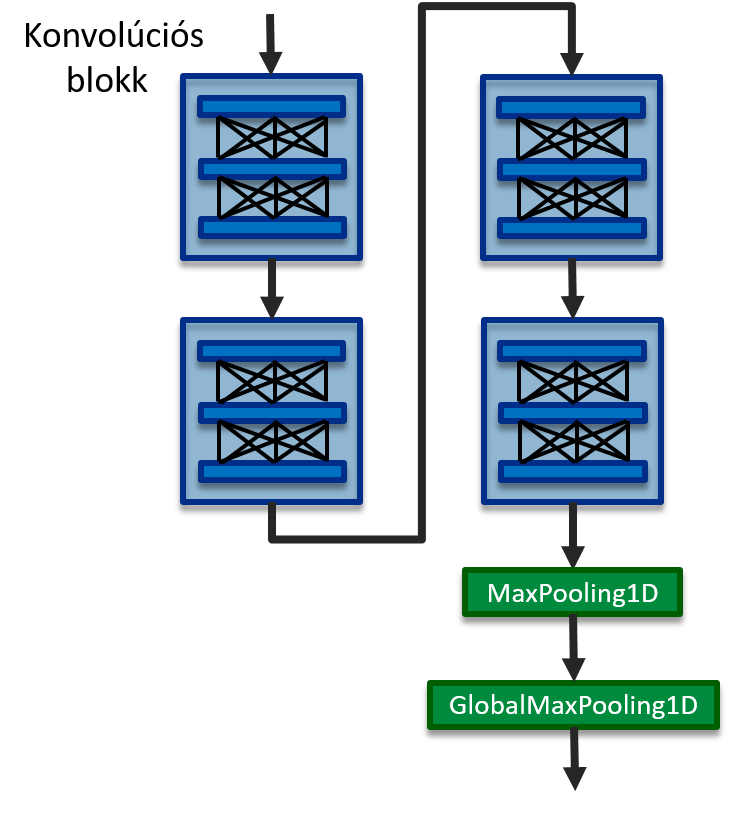
\includegraphics[width=100mm, keepaspectratio]{figures/conv_encoder.png}
	\caption{A konvolóciós enkóder felépítése.}
	\label{fig:conv_encoder}
\end{figure}

A sziámi hálózat alapja két enkóder hálózat, amelynek súlyai megosztottak, tehát úgy is tekinthetünk rá, hogy egy enkóder hálózatra két bemenetet adhatunk. A hangminták a hálózaton áthaladva jellemző vektorokká alakulnak. Ezt a részt a konvolúciós enkóder végzi. Ezután a két vektor közötti távolságmetrikát a sziámi hálózat kiszámolja. Ezen távolság alapján számolja ki a veszteséget és javítja a súlyokat.

Az implementált távolságmetrikák a következők:

\begin{itemize}
	\item \emph{weighted\_l1}: Az eredeti one-shot cikk szerinti távolságmetrika. $v_1$ és $v_2$ vektorokra $\sqrt{v_1-v_2}$.
	\item \emph{uniform\_euclidean}: Euklideszi távolság két vektor között.
	\item \emph{cosine\_distance}: Koszinusz távolság, azaz a két vektor által bezárt szög koszinuszát méri.
\end{itemize}

A kiszámolt távolság ezután minden esetben áthalad egy szigmoid aktivációs függvényű \emph{Dense} rétegen, ami $0$ és $1$ közé nyomja az eredményt.

\subsection{Beszédadatbázisok és generátorok}

A voicemap tanításhoz és teszteléshez a \emph{LibriSpeech} adatbázis \emph{dev-clean}, \emph{train-clean-100} és \emph{train-clean-360} adathalmazokat használja, amelyek sorban $40$, $251$ és $921$ különböző beszélőtől tartalmaznak nyers hangfájlokat.
\newline
\newline
Egy adathalmazt egy adatgenerátor osztály reprezentál ami a keras.util.Sequence osztályból származik. Az adatgenerátorok nagy adathalmazok esetén hasznosak, amikor az egész adathalmaz nem fér bele a memóriába. Ilyen esetekben egyesével generálnak adatokat.
\newline
\newline
A \emph{keras.util.Sequence} osztályból való leszármaztatás miatt az adatgenerátorban implementálni kell a \emph{\_\_len\_\_} és \emph{\_\_get\_item\_\_} függvényeket. Előbbi az adathalmaz méretét adja vissza, utóbbi annak indexelését teszi lehetővé. Továbbá biztosítja, hogy egy epochon belül egy mintával csak egyszer tanítjuk a modellt.

\subsection{Tanítás}

A sziámi és a sima klasszifikációs hálózat nagyrészt közös paraméterekkel rendelkeznek. A fő különbség, hogy míg a sziámi veszteségfüggvénye bináris keresztentrópia, és a veszteség az alapján dől el, hogy a hangminta pár egyazon vagy más beszélőktől származik, a klasszifikációs hálózat kategórikus keresztentrópiát használ, tehát a hangmintát megpróbálja besorolni $k$ osztály valamelyikébe $k$ beszélő esetén. A közös paraméterek:

\begin{itemize}
	\item hangminta hossza: 3 sec
	\item batchsize: 64
	\item filterek száma: 128
	\item jellemző vektor dimenzió: 64
	\item dropout: 0
	\item steps\_per\_epoch: 500
	\item kiértékelési feladatok száma: 500
	\item n\_shot\_klasszifikáció: 1
	\item k\_way\_klasszifikáció: 5
\end{itemize}

Tehát mindkét modell optimizált hiperparamétereket használ, \emph{Adam} optimizálót és veszteségfüggvényként keresztentrópiát. Egy epoch $500$ batch iterációból áll és egy batch méret $64$.
Az epochok végén három callback fut le.
\newline
\newline
Minden epoch végén kiértékelés történik: 500 \emph{1-shot 5-way} feladat átlagos eredménye jelzi a pontosságot. Amennyiben ez növekszik a modellről \emph{checkpoint} készül (\emph{ModelCheckpoint}).
Továbbá ha a kiértékelés során a pontosság nem nő, a \emph{ReduceLROnPlateau} csökkenti a tanulási rátát.


\subsection{Kísérletek és optimalizálás}

A repositoryban számos kísérlet található a legjobb teljesítmény elérésére. A \emph{wide\_vs\_tall} szkript leméri, hogy a modell hogyan teljesít különböző hosszúságú hangmintákkal tanítva. A mérés alatt \emph{1-shot 5-way} feladatokkal, azaz 5 különböző beszélőtől 1-1 beszédmintával validálta a modellt.

\begin{figure}[!ht]
	\centering
	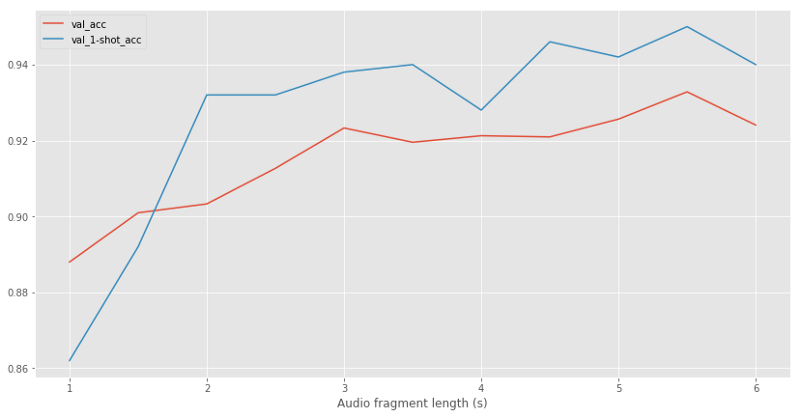
\includegraphics[width=150mm, keepaspectratio]{figures/voicemap-wide-vs-tall.png}
	\caption{Voicemap: Regisztrációs fázis.}
	\label{fig:voicemap-wide-vs-tall}
\end{figure}

A \ref{fig:voicemap-wide-vs-tall} ábrán látható, hogy a hangminta méretét növelve a modell valóban jobban tanul, de a több adat miatt megnövekedik a tanítási idő és több memóriára van szükség. A grafikon mutatja, hogy 3 másodperc után a validáció stagnálni kezd, ezért az erőforrásokat és a tanítási időt figyelembe véve ez tűnik a legjobb választásnak.

A \emph{grid\_search\_siamese\_network} szkript hiperparaméter optimizációt végez a sziámi hálózaton a filterek számát, a hangmintákból képzett vektorok hosszát és a dropoutot vizsgálva. A talált legjobb paraméterek:

\begin{itemize}
	\item filterek száma: 128
	\item jellemző vektor dimenzió: 64
	\item dropout: nincs
\end{itemize}

A \emph{k\_way\_accuracy} kísérlet a hiperparaméter optimalizált modellt teljesítményét méri le különböző \emph{n-shot k-way} feladatokkal. A pontosságot a következő ábra mutatja:

\begin{figure}[!ht]
	\centering
	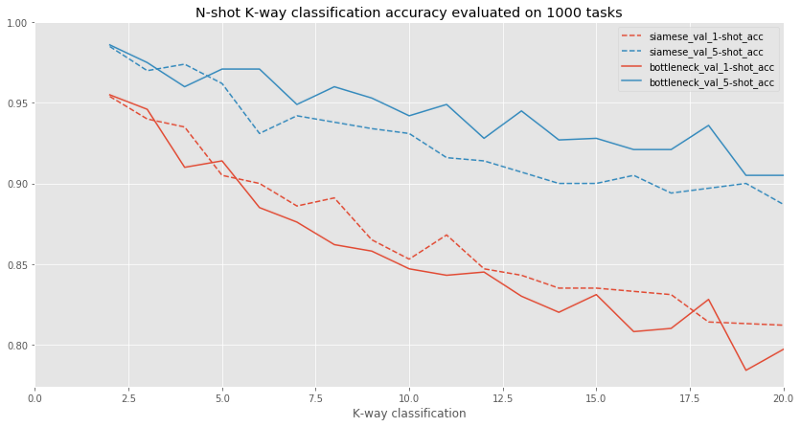
\includegraphics[width=150mm, keepaspectratio]{figures/voicemap-n-shot-k-way.png}
	\caption{Voicemap: n-shot k-way pontosság.}
	\label{fig:voicemap-n-shot-k-way}
\end{figure}

\emph{1-shot k-way} feladatok esetén a sziámi hálózat átlagosan jobban teljesít sima klasszifikációsnál, de \emph{5-shot k-way} feladatok esetén már az utóbbi kerül fölénybe. Ez valószínűleg annak köszönhető, hogy 5 hangminta - beszélő párból a sima osztályozó hálózat már jobban meg tudta tanulni a beszélőket a sziáminál.

\newpage

\subsection{Saját kísérletek}

\subsubsection{Contrastive loss}

\subsubsection{Triplet loss}

Létrehoztam egy bemenetként tripleteket fogadó neurális hálózatot \emph{triplet loss} veszteségfüggvénnyel. Egy bemenet egy olyan hangminta hármas (triplet), ami két azonos és egy különbözőtől beszélőtől tartalmaz hangmintát. 
\newline
\newline
A két azonos minta közül az egyik lesz az \emph{anchor} érték. Ehhez mérten számoljuk ki a pozitív (azonos beszélőtől származó) és negatív (különböző beszélőtől származó) távolságokat. 
\newline
\newline
Az alapja a konvolúciós enkóder. Ehhez csatlakozik három bemenet, a kimenetére pedig két lambda réteg ami a pozitív és negatív távolságokat számolja ki, majd még két lambda réteg kiszámolja a vektorok hosszát. A szubtrakciós réteg a ezután a két kiszámolt vektort kivonja egymásból, ahogy a \ref{fig:triplet-network} ábrán látható.

\begin{figure}[!ht]
	\centering
	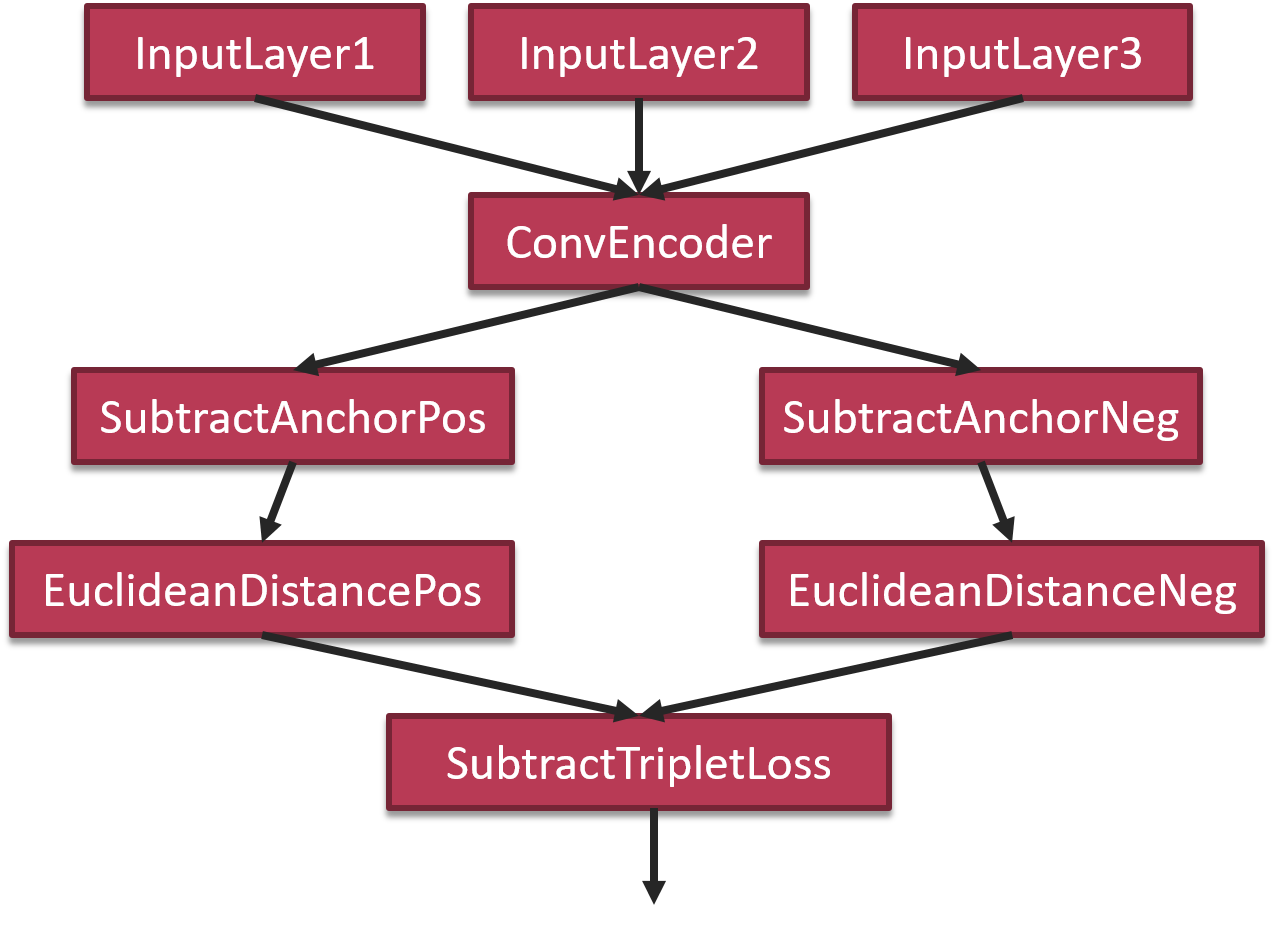
\includegraphics[width=120mm, keepaspectratio]{figures/triplet-network.png}
	\caption{Triplet hálózat.}
	\label{fig:triplet-network}
\end{figure}